\chapter{Dataset and Workload Analysis}\label{chp:dataset}

In recent years, an emerging trend within the research community has been a shift from traditional scheduling approaches (e.g., FIFO) toward SJF. The purpose of this chapter is to describe the dataset utilized throughout this thesis; the steps taken to clean, prepare, and transform the data for modeling; the exploratory data analysis (EDA) that informs several critical design choices; and the feature extraction process that converts raw job logs into model-ready input formats. All analyses are based on the open-source Alibaba PAI GPU cluster trace~\cite{weng2022mlaas}.

%% ================================================================
\needspace{5\baselineskip}
\section{The Alibaba PAI GPU Cluster Dataset}

The Alibaba PAI GPU cluster trace was collected from a production cluster that was running on Alibaba's PAI~\cite{weng2022mlaas}. This cluster has about 1,800 machines equipped with a total of more than 6,500 GPUs. These are used continuously and heterogeneously for both internal and external customer ML training and inference workloads.

The raw trace has 100,000 job records sent over a roughly eight-day period. Each job record contains the following attributes: a unique job identifier (\texttt{job\_id}), the timestamp at which it was submitted (\texttt{arrival\_time}), the number of GPUs requested (\texttt{gpu\_demand}), the number of CPUs requested (\texttt{num\_cpu}), the number of parallel instances (\texttt{num\_inst}), the hardware type of the GPU (\texttt{gpu\_type}), and the user who submitted it (\texttt{user}). The primary prediction target is the job runtime (\texttt{job\_runtime}), or the total number of seconds the job ran after it was submitted until it completed.

%% ================================================================
\needspace{5\baselineskip}
\section{Data Cleaning and Preprocessing}

Raw trace files have a variety of forms of noise and inconsistencies to correct prior to training predictive models. The processing pipeline performs the following:

\textbf{Removing missing values.} Any record with a missing value for the \texttt{job\_runtime} field will be removed from the pre-processed data. Most of these records are jobs which were canceled before executing or jobs that failed to log.

\textbf{Filtering for no GPUs.} All job requests with zero GPUs will be removed. These records are not included within the scope of this thesis. There is no need to include them in decision-making processes for GPU scheduling.

\textbf{Filtering out non-positive runtimes.} Records with a runtime of zero or a negative duration will be removed. These records are logging artifacts instead of actual workloads.

After removing invalid records, the processed dataset has \textbf{82,184 valid GPU jobs} remaining from the 100,000 original records. All 17,816 eliminated records were removed by the zero-GPU filter: they carry \texttt{gpu\_type} = \texttt{CPU} and request no GPU at all. The missing-runtime and non-positive-duration filters are applied for robustness but removed no record from this sample, since every entry in the trace reports a strictly positive duration. A single CSV file will serve as a deterministic data source for all further analysis, modeling, and simulation.

%% ================================================================
\needspace{5\baselineskip}
\section{Exploratory Data Analysis}

Prior to developing predictive models based on the workload, an EDA is performed to establish knowledge about the statistical characteristics of the workload. All modeling and scheduling activities are grounded in the results presented below.

\subsection{Runtime Distribution}

Job durations show extreme variability with what is called the ``mice and elephants'' effect. Most jobs (or ``mice'') have a median duration of about 10 minutes (594 seconds) with the upper quartile (i.e., the 75th percentile) being just slightly greater than 1 hour. However, a small number of jobs (or ``elephants'') last for days, resulting in a very long maximum duration of nearly seven days. In addition, the distribution of job durations is highly asymmetric to the right, confirming that there are many short-duration jobs used for interactive tasks or testing purposes; however, these make up only a small fraction of total resource utilization compared to the few long-duration distributed training runs that consume most of the available resources over time.

In addition to its asymmetry, we see from the coefficient of variation that the distribution has a high degree of dispersion relative to its central tendency. Thus, standard mean-based statistical models combined with common loss functions (such as MAE) will be poorly suited to model the observed variance. These two characteristics highlight the importance of ``decision-focused'' runtime predictions: if all jobs were treated equally by applying a FIFO policy to them, it could result in severe HoL blocking where one or a few ``elephant'' type jobs can delay the execution of hundreds of ``mouse'' type jobs.

\clearpage
A plot showing both the raw and log-transformed distributions of job durations is shown in Figure~\ref{fig:runtime-dist}. In the left panel, we display the raw distribution of job durations. We see that there is a great deal of rightward skewness present: nearly all job times fall within the 0-20,000\,s interval. There is also a long tail extending into the approximate region of 600,000\,s. To better visualize the distribution, we apply a log\textsubscript{10} transformation to each value in the dataset and then plot it as well. The rightmost panel displays this transformed distribution. As shown in the figure, we now clearly observe a bimodal structure with two separate maxima. The primary peak occurs at log\textsubscript{10}~$\approx$~2.5 ($\approx$300\,s), suggesting that there is an abundance of short-duration jobs used primarily for inference-type applications or rapid debugging jobs. Additionally, we find that a second, albeit smaller peak exists at log\textsubscript{10}~$\approx$~4.0 ($\approx$10,000\,s), indicative of longer duration ML training operations. The existence of a clear bimodal structure in this dataset supports our previous assertion that the cluster hosts two significantly different types of application workloads, and further reinforces our decision to employ a log\textsubscript{10} transformation to visualize the distribution, revealing the complex bimodal nature of the raw runtime data that our predictive models must learn to estimate.

\begin{figure}[htbp]
\centering
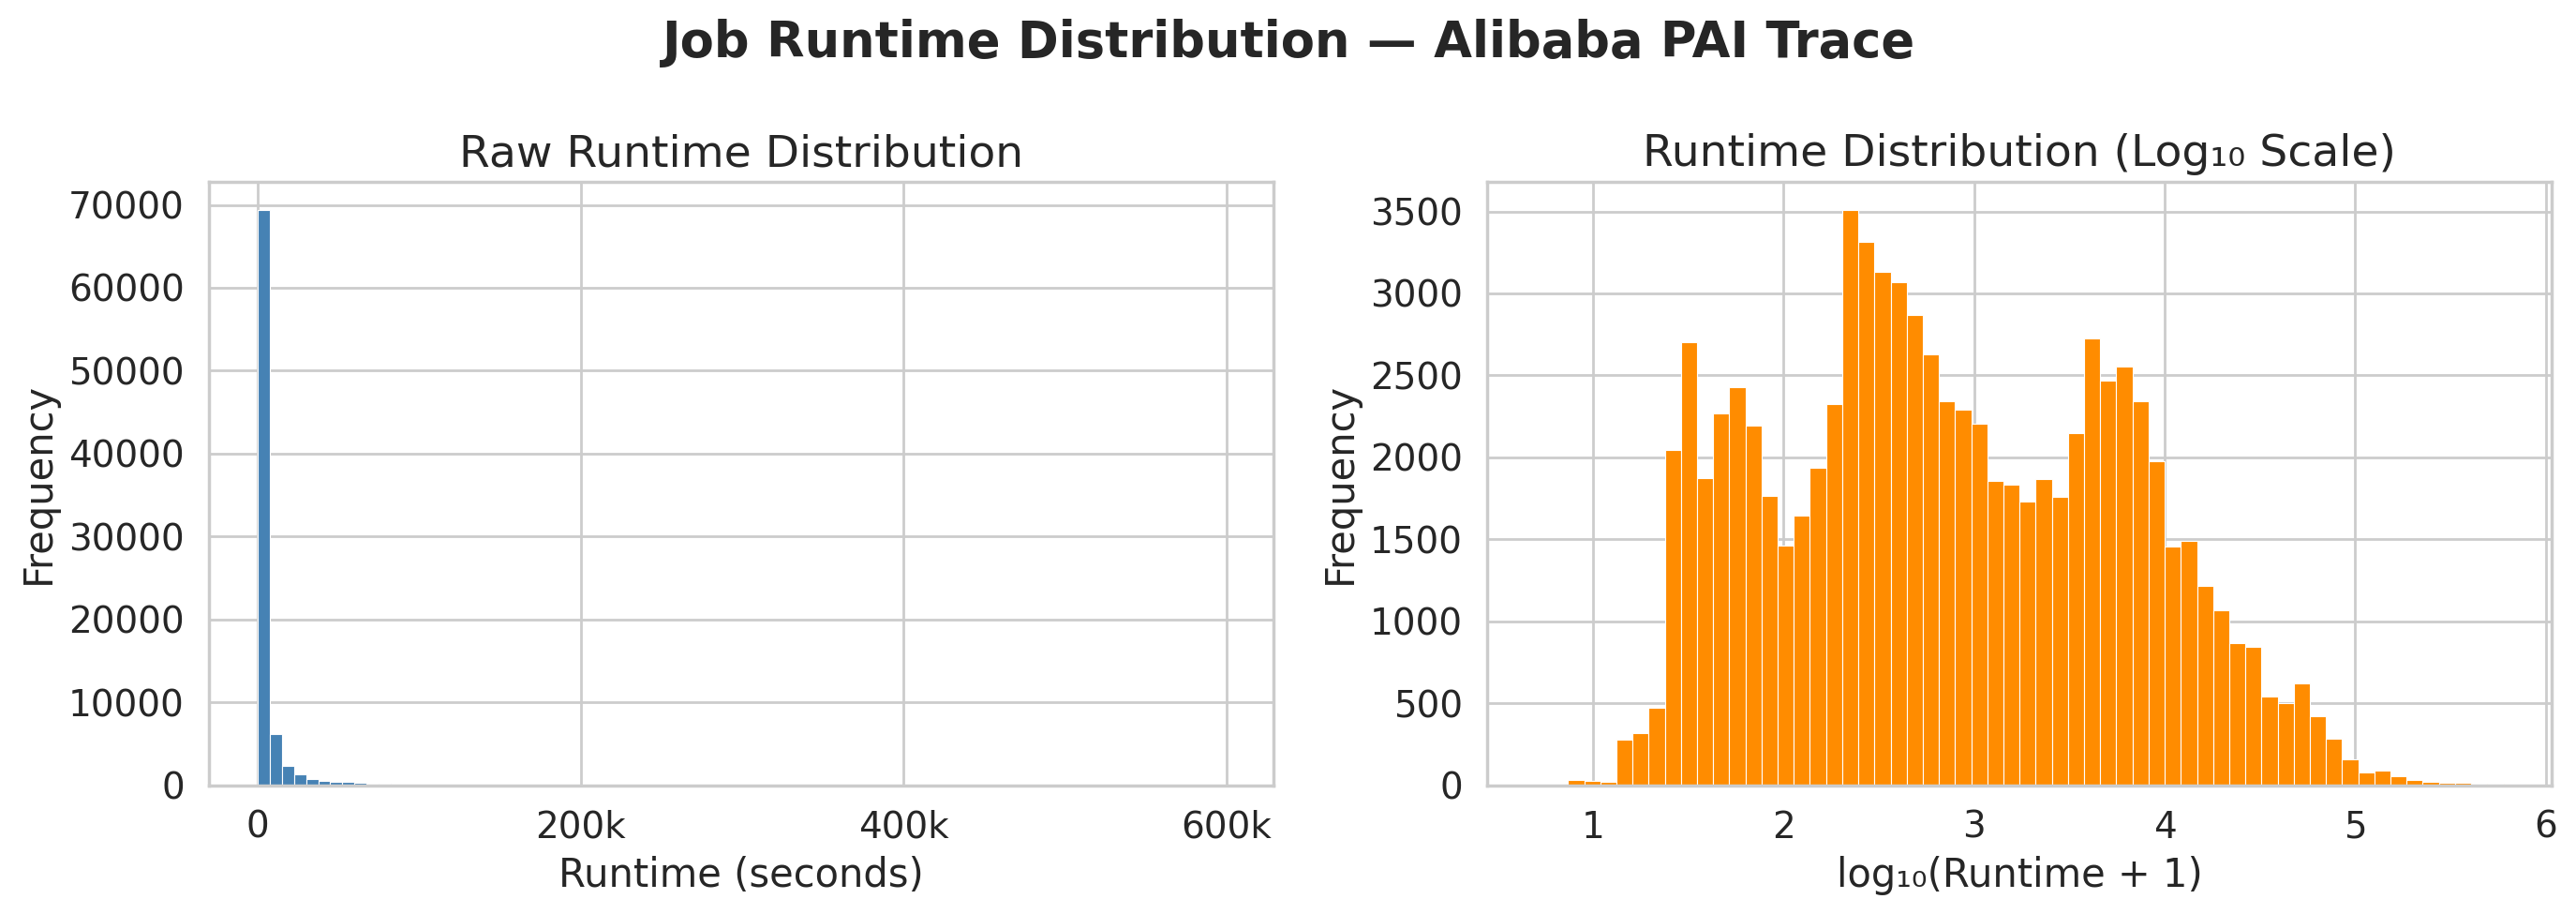
\includegraphics[width=\textwidth]{figures/nb01-fig01-runtime-dist.png}
\caption[Job runtime distribution]{Distribution of job runtime (in seconds), both in raw scale (left) and in log\textsubscript{10} scale (right). Due to extreme skewness toward long job durations, we observe a clear difference between the two visualizations. While the log\textsubscript{10} scale provides insight into the shape of the distribution, it clearly indicates the presence of two distinct modes. We can identify these as job runtimes around 300\,s and those in excess of 10,000\,s.}
\label{fig:runtime-dist}
\end{figure}

\newpage
Figure~\ref{fig:runtime-cdf}, shown with a logarithmic scale on the x-axis, illustrates the cumulative distribution function (CDF) of job runtimes. A steep increase at the beginning confirms that almost all of the jobs finish rapidly; however, the long and flat tail indicates that although they represent a small percentage of the total number of jobs, there exists a significant amount of extremely long-running ML training jobs. Percentiles of interest may be obtained from the CDF: P50 (median) = 594\,s ($\approx$10 minutes), P95 = 24,110\,s ($\approx$6.7 hours), and P99 = 67,432\,s ($\approx$18.7 hours). A ratio of about 40.6 for P95/P50 demonstrates an untypically large coefficient of variation, indicating that this is a difficult regression objective. From a scheduling perspective, the extreme heavy tail demonstrated by this dataset means that FIFO-based ordering will likely be highly susceptible to HoL blocking, as a single multi-day ML training job has the potential to stall hundreds of short interactive jobs behind it.

\begin{figure}[htbp]
\centering
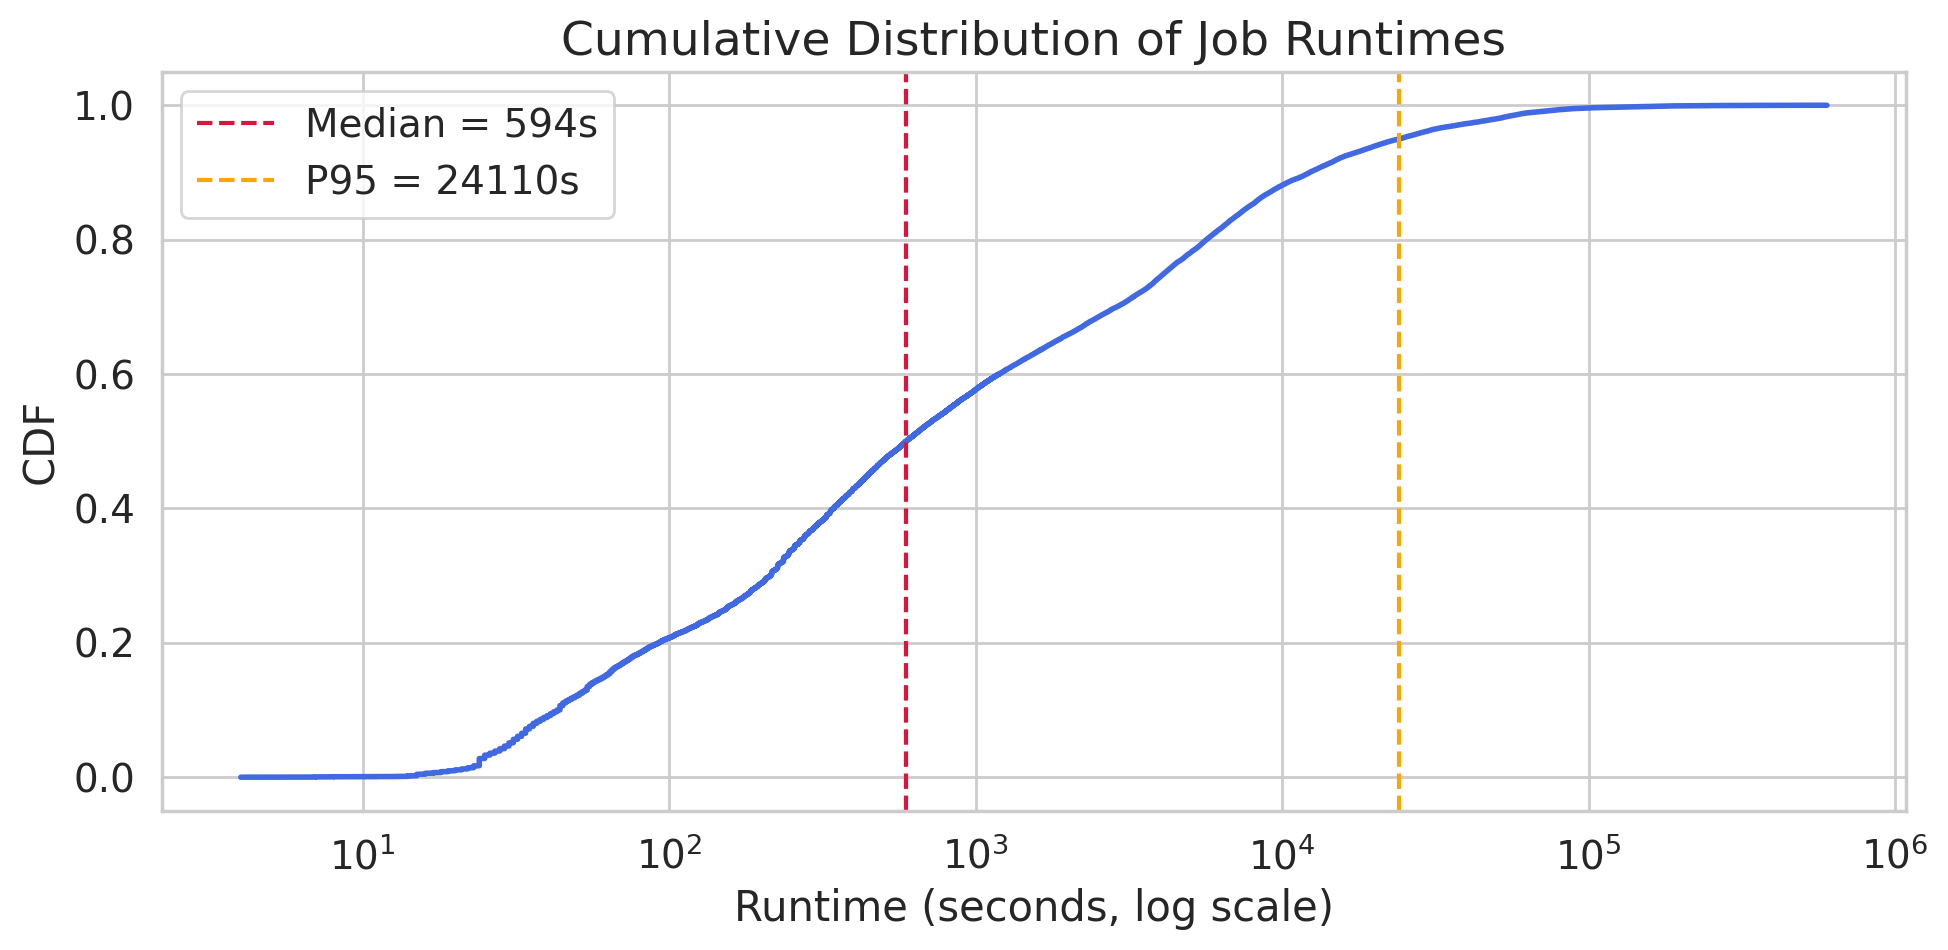
\includegraphics[width=0.85\textwidth]{figures/nb01-fig02-runtime-cdf.png}
\caption[Runtime CDF]{Cumulative distribution function of job runtimes. The x-axis is log-scaled. Key percentiles: P50 = 594\,s, P95 = 24,110\,s, P99 = 67,432\,s.}
\label{fig:runtime-cdf}
\end{figure}

\clearpage
\subsection{Resource Request Heterogeneity}

Figure~\ref{fig:gpu-demand} illustrates the variation in GPU demand among jobs submitted to the PAI cluster, as evidenced by the wide variety of resource requests. Of all jobs, the approximately 37,000 jobs requesting one or fewer GPUs formed the most prevalent category. Requests for multiple GPUs were much less frequent than single-GPU requests and appear as a ``long tail''. With an average demand of 0.52 GPUs across the selected jobs, the highest possible number of GPUs demanded at once was 8. These differing demands justify including \texttt{gpu\_demand} as a key predictor variable for the regression models, and support the use of multiple node profiles within the scheduling simulator (Chapter~\ref{chp:simulation}).

\begin{figure}[htbp]
\centering
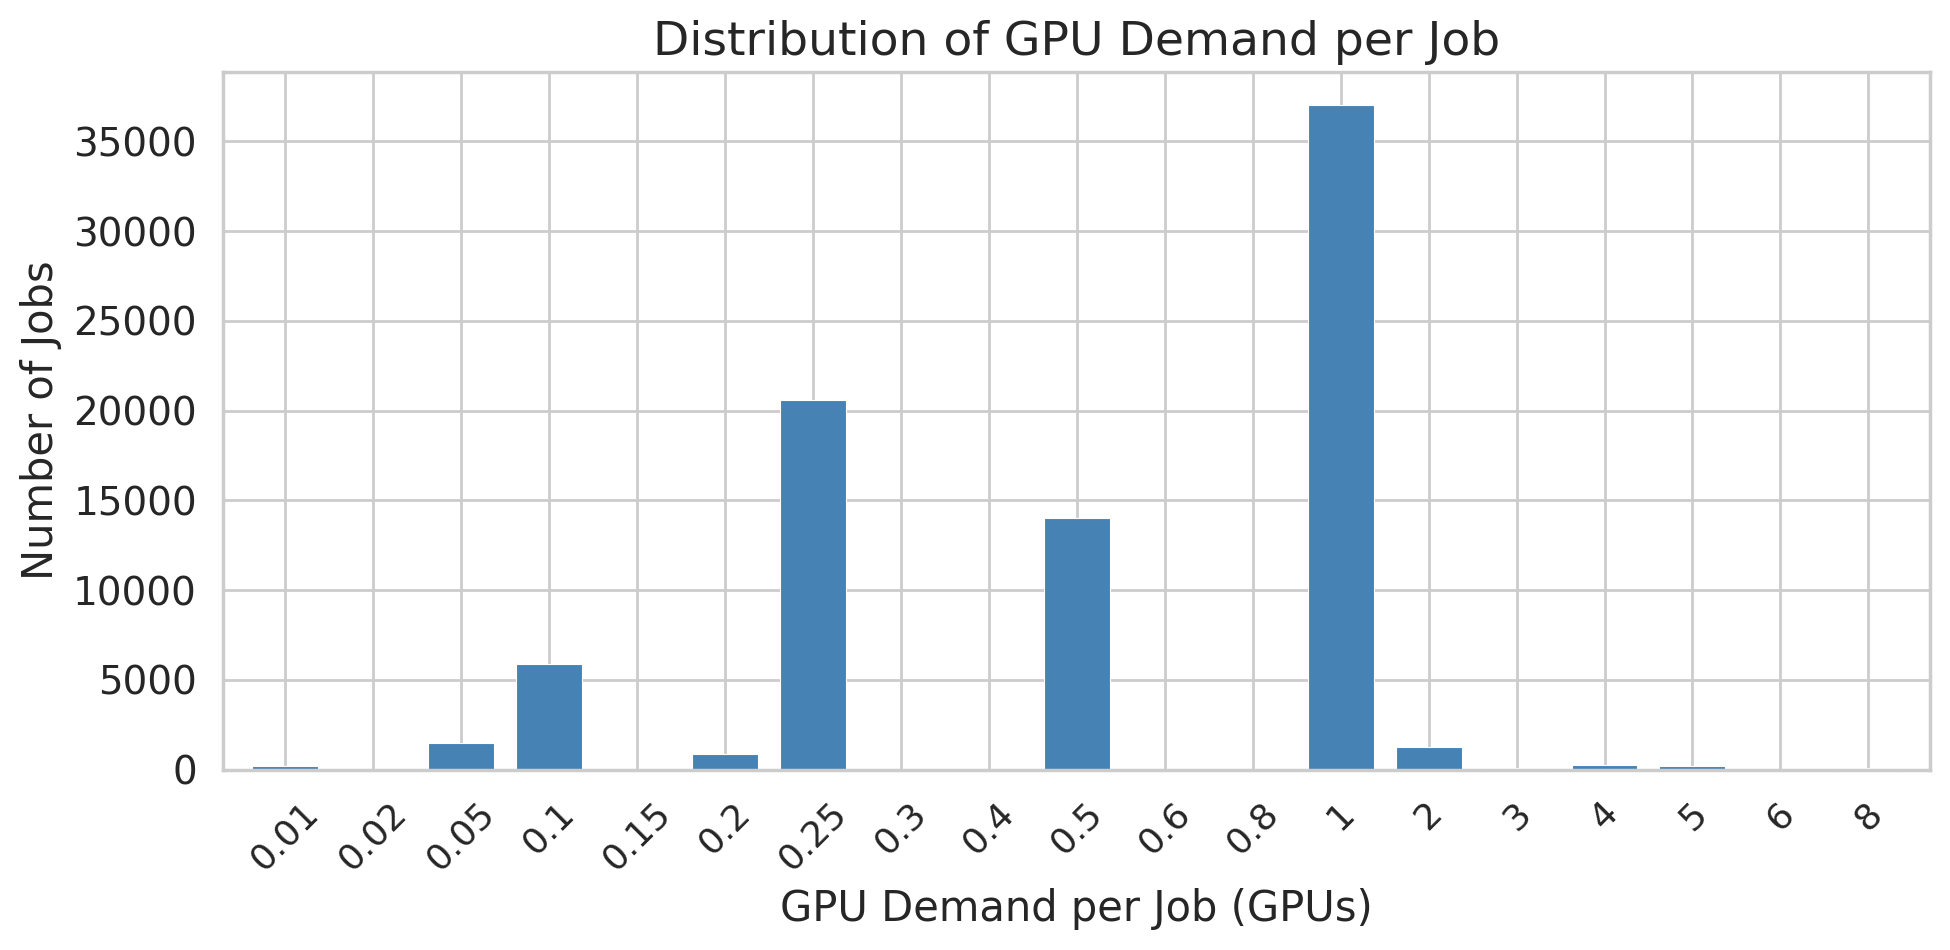
\includegraphics[width=0.75\textwidth]{figures/nb01-fig04-gpu-demand.png}
\caption[GPU demand per job]{Histogram of the number of GPUs requested per job. It is evident that almost every request is for a single GPU. Multi-GPU requests (2-8) occur rarely; however, they require an overwhelming amount of cluster resources.}
\label{fig:gpu-demand}
\end{figure}

\clearpage
Figure~\ref{fig:gpu-vs-runtime} shows the connection between GPU requests and runtime for jobs, using 5,000 randomly selected samples, with both axes on a log scale. The scatter plot shows no simple linear correlation between GPU requests and runtime. The jobs that used a single GPU had runtimes ranging from 10\textsuperscript{1}\,s to 10\textsuperscript{5}\,s ($\approx$10\,s to $\approx$28\,hours). Higher GPU requests (6-8 GPUs) are rare but appear close to the 10\textsuperscript{4}\,s mark. This confirms that \texttt{gpu\_demand} alone is fundamentally insufficient for accurate runtime prediction, motivating the addition of other context-based features like \texttt{user}, \texttt{gpu\_type}, and cluster utilization metrics.

\begin{figure}[htbp]
\centering
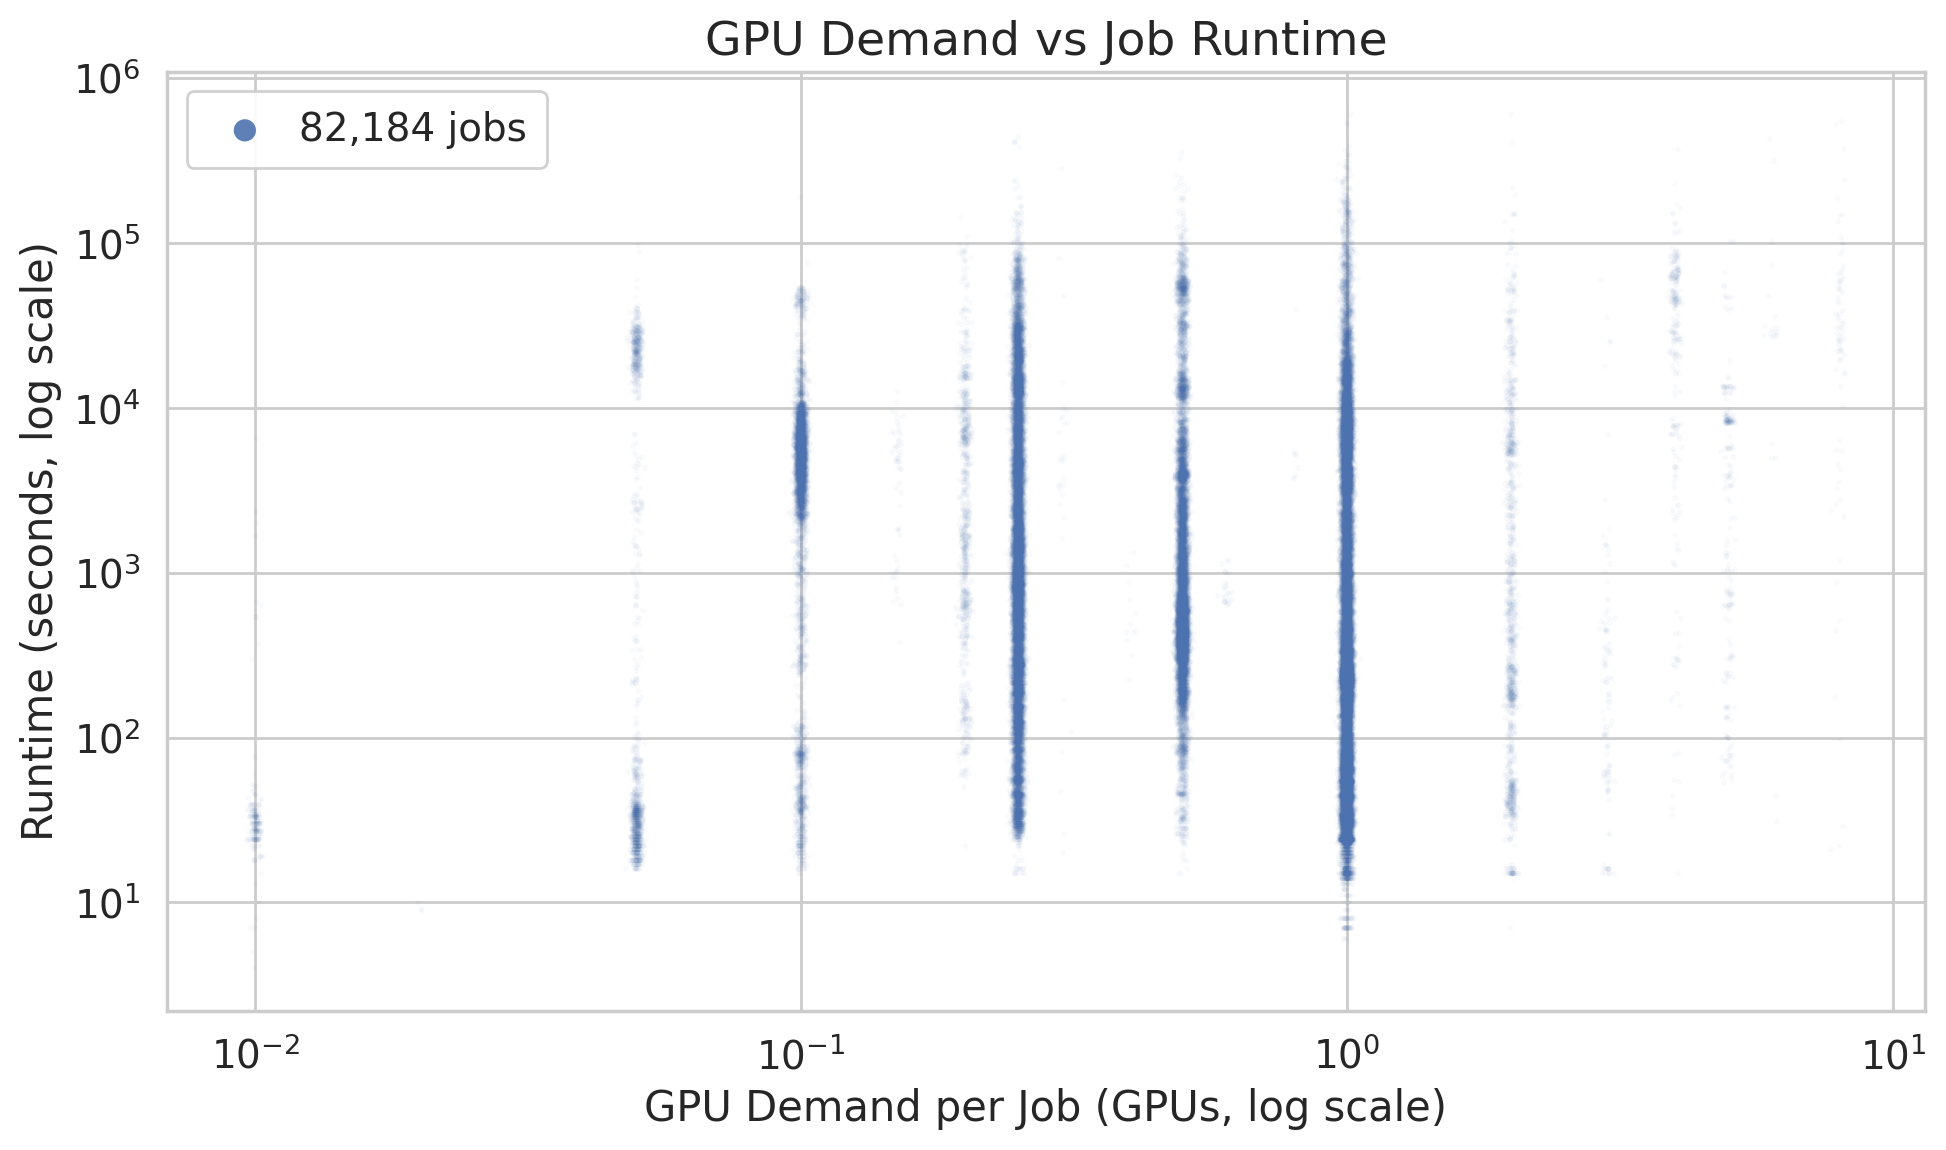
\includegraphics[width=0.75\textwidth]{figures/nb02-fig03-gpu-vs-runtime.png}
\caption[GPU demand vs runtime scatter]{Scatter plot of GPU demand versus job runtime (5,000-job sample, log scale). The large variability within each GPU class is evidence that the GPU demand of a job alone does not determine its runtime.}
\label{fig:gpu-vs-runtime}
\end{figure}

\clearpage
\subsection{Temporal Submission Patterns}

Figure~\ref{fig:arrival-rate} shows the hourly average arrival rates for the entire trace (8 days). This figure clearly illustrates that user-submitted jobs exhibit a clear daily cycle which is consistent with users submitting workloads throughout their working hours, whereas automated batch systems do not produce such cycles. It is important to remember that the times of submissions for all items in this dataset were obtained as normalized UNIX timestamps. Therefore, while the hour-of-day values represent UTC time, they will not be the actual time at which a user submitted an item to their cluster (the hourly pattern may vary slightly by cluster based on daylight savings or other temporal events). Nonetheless, the weekly and daily cyclicality patterns of submission relative to these hours will still be correct. The baseline job submission rate is generally about 200-400 jobs/hour but there have been several larger spikes in job submissions; most notably at 1,350 jobs/hour for day~1.5 and at 1,050 jobs/hour for day~5.5. Shorter-term increases such as this can quickly lead to queue backlogs that require an efficient method to order queued jobs by the scheduler during these periods. Due to the periodic nature of the peak arrivals, the assumption of a stationary Poisson process that is often made in traditional queueing models does not apply.

\begin{figure}[htbp]
\centering
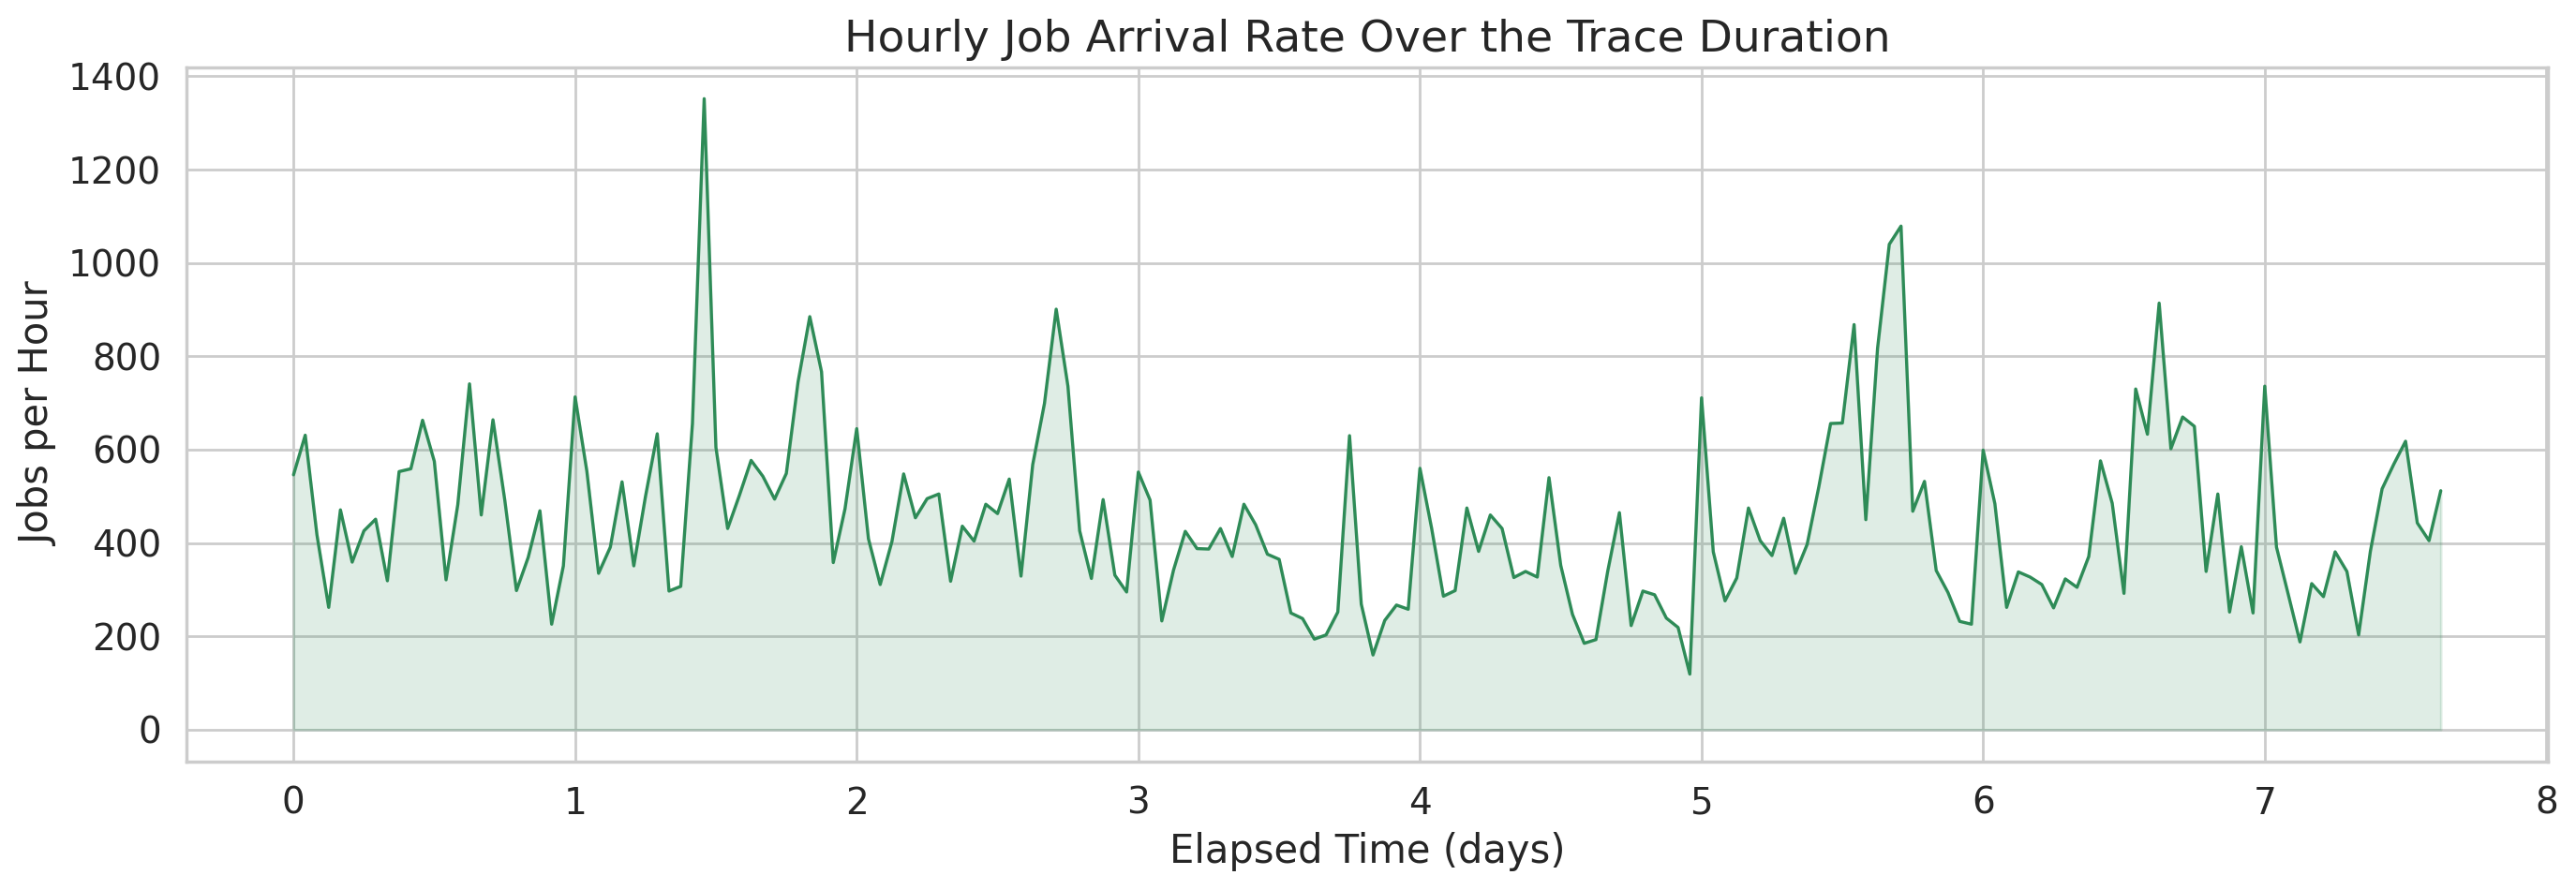
\includegraphics[width=\textwidth]{figures/nb01-fig03-arrival-rate.png}
\caption[Hourly arrival rate]{Hourly job submission rates during the 8-day trace. There is a baseline submission rate of 200-400 jobs/hour with occasional transient increases above 1,000 jobs/hour.}
\label{fig:arrival-rate}
\end{figure}

\clearpage
Figure~\ref{fig:interarrival} represents the distribution of time intervals (in seconds) between each pair of jobs submitted to the scheduler. This distribution is presented with a logarithmic scale on the x-axis. The large peak at the 1-3\,s bin ($\approx$25,000 jobs) indicates that most jobs arrive back-to-back as bursts. After a sharp decrease in frequency, there are $\approx$8,000 jobs arriving within the next 3-10\,s interval. Inter-arrival times longer than 100\,s occur extremely infrequently. The significant skewness of this distribution clearly shows that the arrival process does not follow an exponential pattern. Therefore, standard single-server queueing models based on the $M/M/1$ model cannot be used to characterize this type of workload. As a result of burst arrivals, where multiple jobs arrive within seconds, both the duration of queueing delay and the probability of queueing delay are significantly influenced by the workload dynamics. Therefore, during dynamically changing loads (bursts), scheduling based on SJF is significantly more effective than FIFO.

\begin{figure}[htbp]
\centering
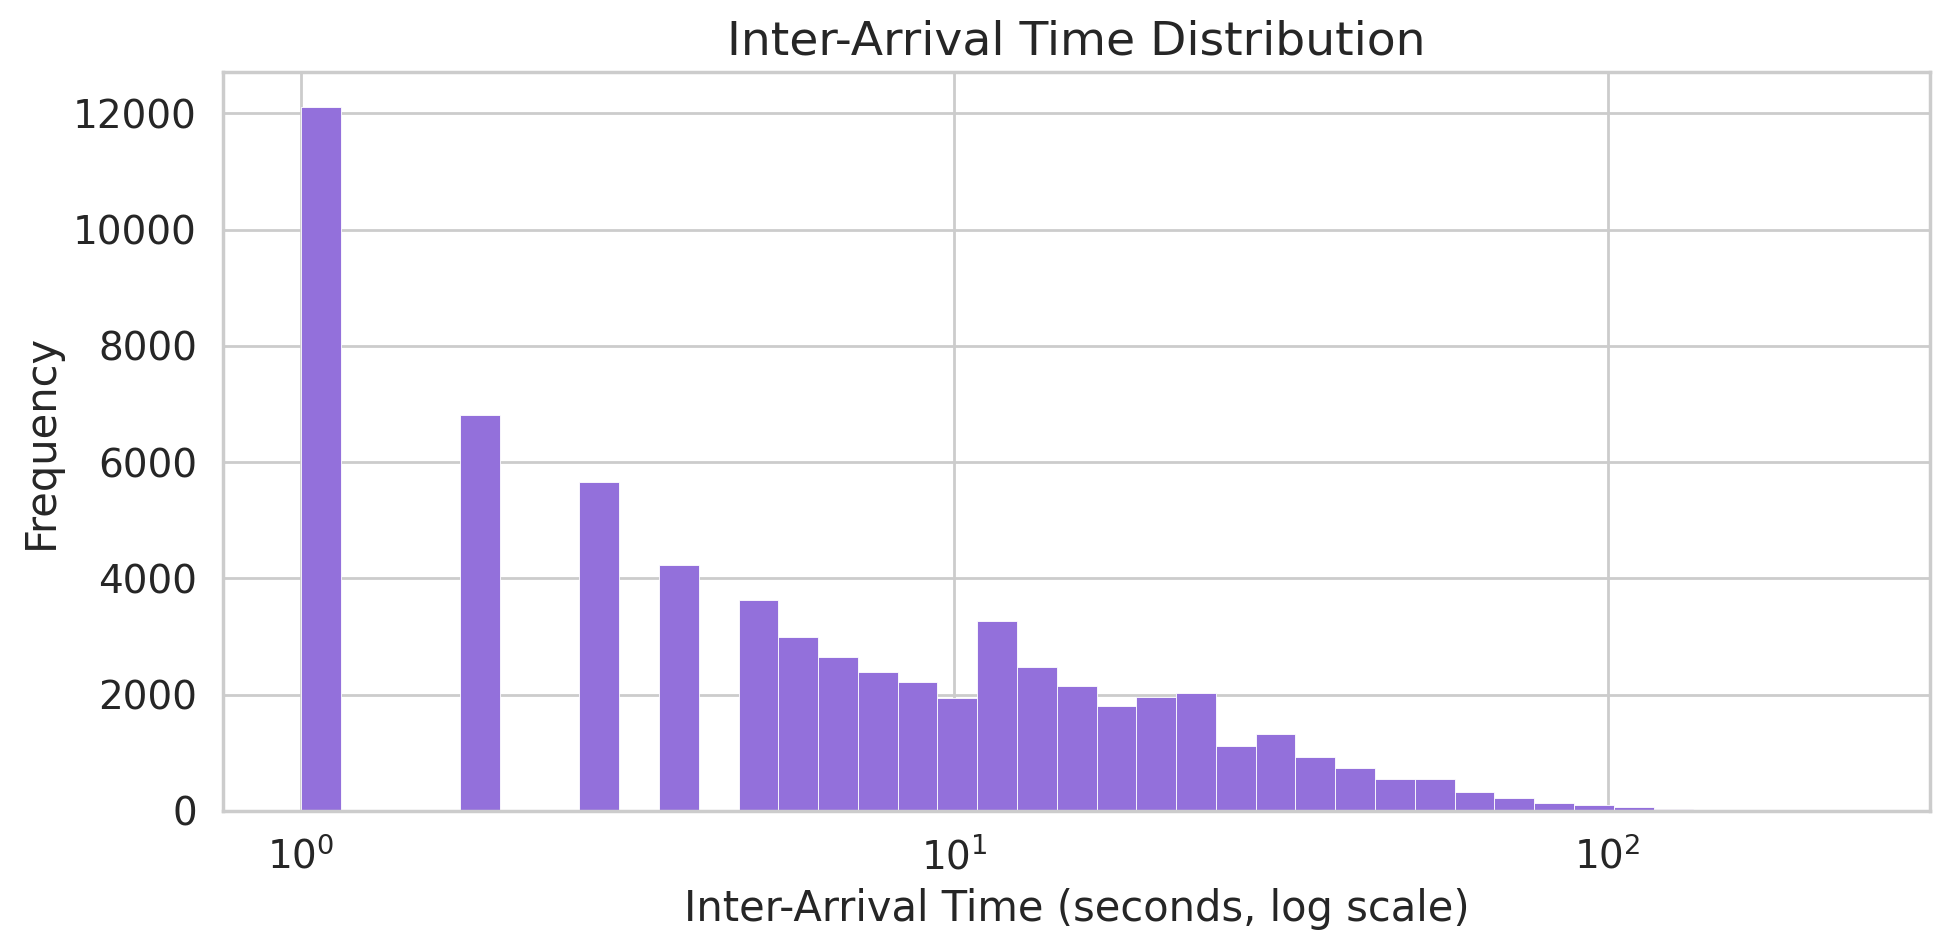
\includegraphics[width=0.75\textwidth]{figures/nb01-fig05-interarrival.png}
\caption[Inter-arrival time distribution]{Logarithmic histogram of inter-arrival time between consecutive job submissions. This provides further proof that job submissions have a bursty pattern. The peak occurs at the short time interval of 1-3\,s.}
\label{fig:interarrival}
\end{figure}

\clearpage
Figure~\ref{fig:arrival-heatmap} provides a trace-day by hour-of-day analysis for job submissions. The color intensity of each cell indicates the number of jobs submitted. An earlier draft of this section read the y-axis as calendar days of the week and reported a Monday-through-Friday daytime peak with the heaviest submissions on ``Thursday.'' That reading does not hold: the publicly released trace does not disclose its actual collection date, and it spans only about 7.7 days, so a true calendar-weekday encoding would fold the trace's first and eighth day onto the same value -- unverifiable given the undisclosed start date, and a leakage risk for the chronological train/test split, since every training occurrence of that shared value would come from the trace's first day while every test occurrence comes from its last. \texttt{day\_of\_week} is therefore computed as an absolute trace-day counter (0, 1, 2, \ldots) rather than a calendar weekday. The heatmap still shows clear diurnal structure -- daytime hours consistently carry heavier submission volume than late-night hours across the trace's days -- which motivates keeping \texttt{hour\_of\_day} and \texttt{day\_of\_week} as predictive variables, but the figure should not be read as evidence of a specific weekly (Monday-Sunday) pattern.

\begin{figure}[htbp]
\centering
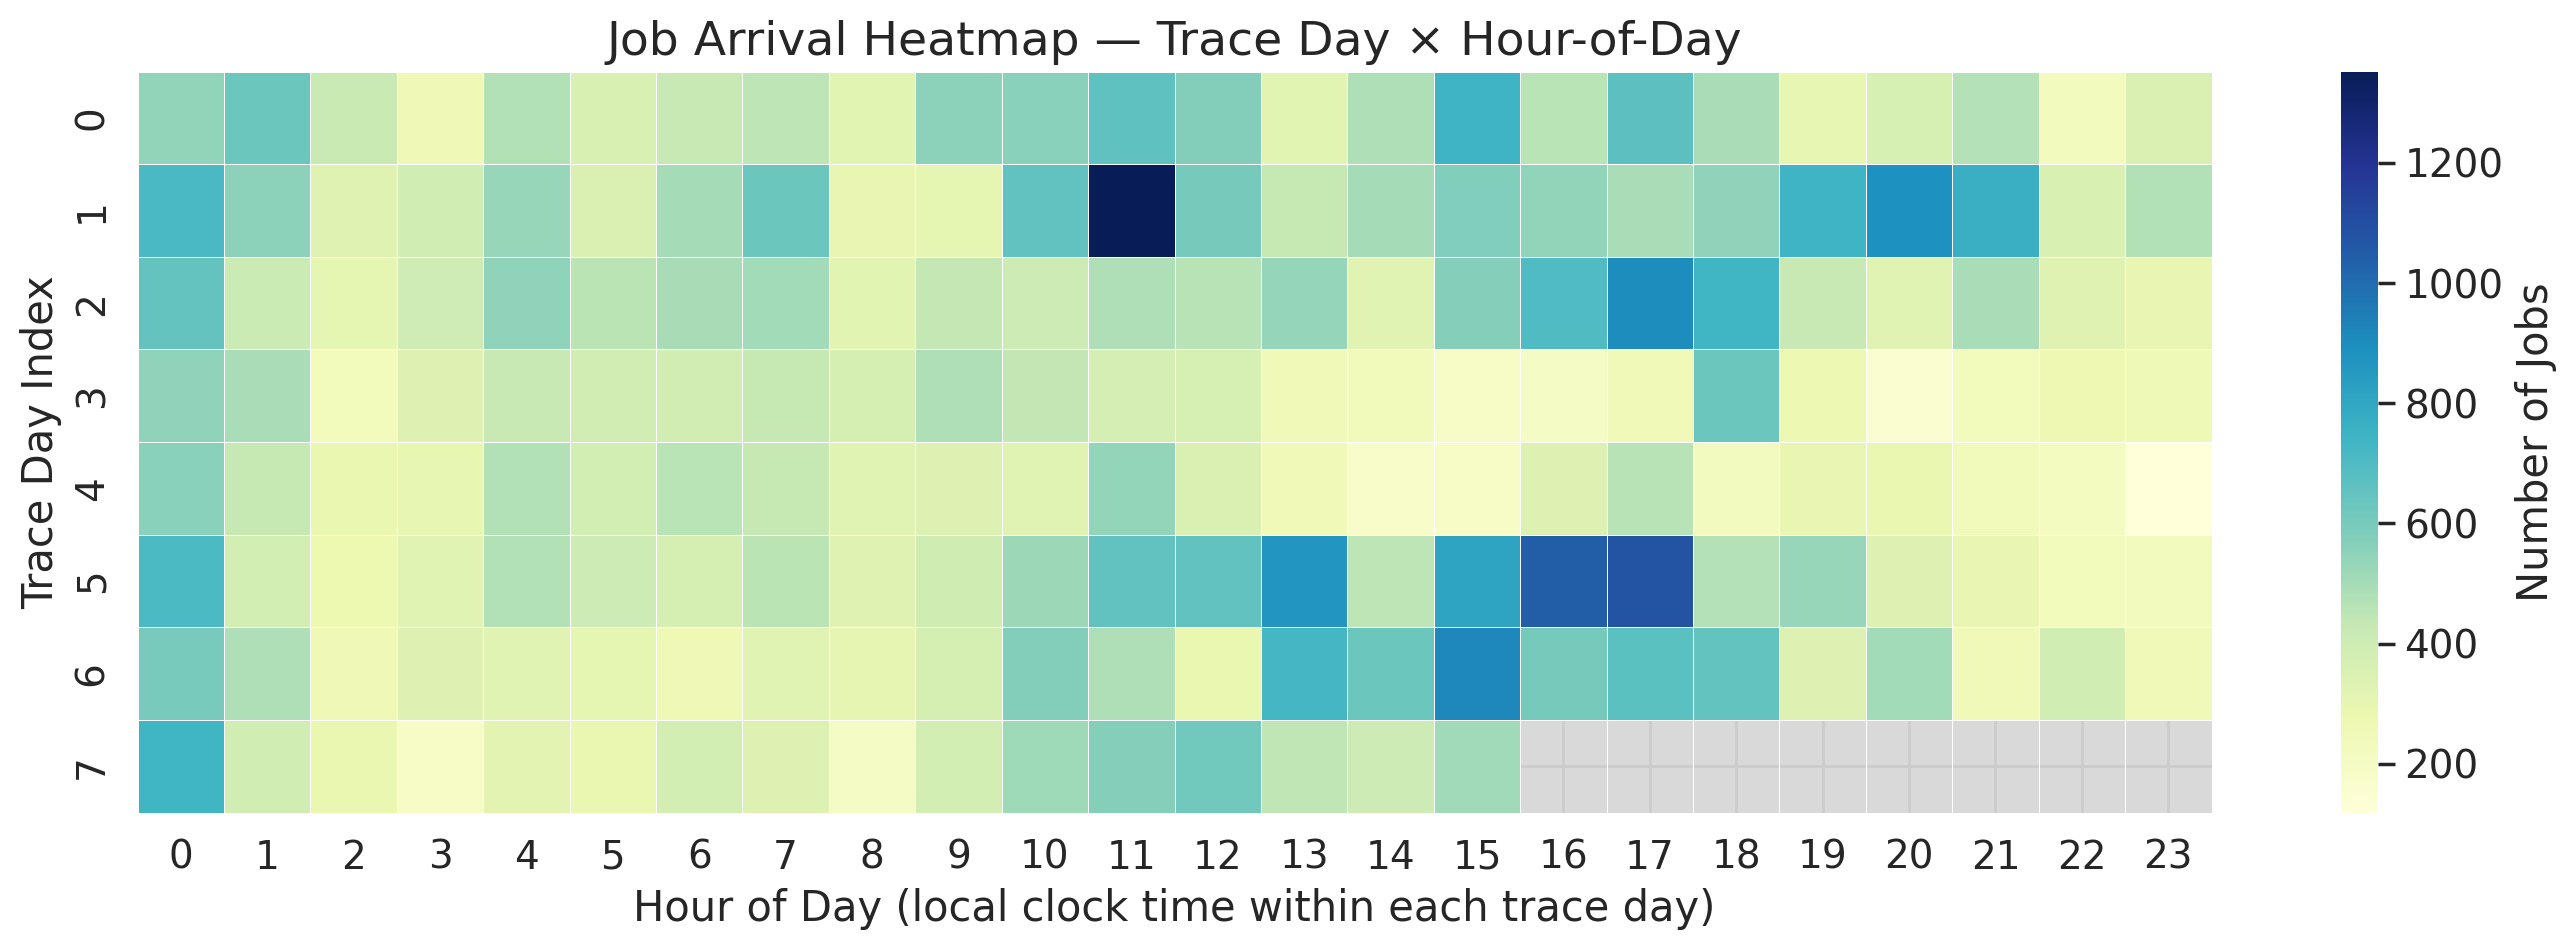
\includegraphics[width=0.75\textwidth]{figures/nb01-fig06-arrival-heatmap.png}
\caption[Job arrival heatmap]{Heatmap of job arrivals per hour of the day and per trace-relative day index (day 0 = the trace's first day). The color intensity corresponds to the number of jobs submitted. Daytime hours appear to be the most concentrated period for job submissions across the trace's $\sim$7.7 days; the y-axis is a trace-day counter, not a calendar weekday (see main text).}
\label{fig:arrival-heatmap}
\end{figure}

%% ================================================================
\clearpage
\needspace{5\baselineskip}
\section{Feature Engineering}

A clean dataset provides raw job characteristics; however, these raw values do not represent the changing environment for each individual job. The feature engineering pipeline has been developed to create a variety of new features which enhance the understanding of each job through temporal, cluster-level, and categorical information.

\subsection{Temporal Context Features}

Submission timing for jobs is very much related to human behavior: jobs are most often submitted during peak working hours, then drop off significantly overnight. Submission volume also varies from one day of the trace to the next, though the public trace release does not disclose its actual collection date, so this day-to-day variation cannot be attributed to a specific calendar weekday. Temporal features have been created based on the submission timestamp for each job to capture both patterns:

\begin{itemize}
    \item \texttt{arrival\_sec}: Time jobs arrive in the trace in relation to the start time. This produces a continuous time signal for tracking each job's position in the timeframe of the trace.
    \item \texttt{hour\_of\_day}: The hour of the day that a job is submitted; this is determined from the Unix timestamp.
    \item \texttt{day\_of\_week}: An absolute, trace-relative day counter (0, 1, 2, \ldots) indicating which day of the roughly 7.7-day trace a job was submitted on -- not a calendar weekday. A true calendar-weekday encoding would fold the trace's first and eighth day onto the same value, which the undisclosed collection date makes unverifiable and which would introduce a leakage risk into the chronological train/test split (see the Limitations discussion in Chapter~\ref{chp:conclusion}).
\end{itemize}

These allow the models to recognize that both submission behavior and runtime distribution vary in a predictable manner throughout the day and across the trace.

\clearpage
\subsection{Resource Request Features}

All raw resource request fields were taken directly into the feature set so that the models could capture the computing requirements of each job:

\begin{itemize} 
    \item \texttt{gpu\_demand}: Number of GPUs requested.
    \item \texttt{num\_cpu}: Number of CPUs requested.
    \item \texttt{num\_inst}: Number of parallel instances running.
\end{itemize}

\subsection{Sweep-Line Cluster Utilization Features}
\label{sec:sweepline}

A key contribution of this thesis is the development of real-time cluster utilization features based on the current utilization (i.e., the load) of the cluster at the exact time a new job is submitted to the system. These features are determined by applying a sweep-line algorithm to the job timeline.

A sweep-line algorithm processes all events chronologically. For each job there are two types of events in the timeline: a \textit{start} event which occurs when a job is first submitted to the system and an \textit{end} event when the job completes. When processing each \textit{start} or \textit{end} event for a job, the algorithm will increment or decrement counter variables representing how many jobs are currently running, how many CPUs have been assigned, and how many GPUs have been assigned. At the exact moment each job is submitted, these three variable states are stored as the following three usage features:

\begin{itemize}
    \item \texttt{active\_job\_count}: The number of jobs being processed in the cluster at the time of submission. This is the best way to gauge the level of congestion inside the cluster.
    \item \texttt{cluster\_load\_gpu}: The total number of GPUs needed for all currently running jobs. This indicates how intensely GPUs are being contested.
    \item \texttt{cluster\_load\_cpu}: The total number of CPUs required by all currently running jobs. There is an assumption made here: jobs submitted when there are high levels of CPU usage will take longer. The validation of this comes later.
\end{itemize}

Let $J = \{j_1, j_2, \ldots, j_n\}$ be the set of all jobs. Each job $j_i$ will have two values associated with it: the time when it was submitted ($s_i$) and the time when it finished ($e_i$). The concurrent job count for job $j_k$ can be defined as follows:

\begin{equation}
    c_k = \left| \{ j_i \in J : s_i \leq s_k < e_i,\ i \neq k \} \right|
\end{equation}

The sweep-line algorithm can compute $c_k$ for all jobs simultaneously in $O(n \log n)$ time (dominated by the sort operation), which makes it feasible to run on the large number of jobs available in the Alibaba trace.

In Figure~\ref{fig:cluster-load}, we show the time series data collected for the active job count and cumulative GPU allocation during the 8-day trace. The top plot displays the number of active jobs in the system as a function of time, while the bottom plot shows the cumulative GPU allocation as a function of time. During peak periods, the number of active jobs erupts from a baseline of approximately 400 to bursts exceeding 1,000 concurrent jobs. The cumulative GPU demand closely shadows these fluctuations, peaking near 800 simultaneous GPU allocations. It is clear that daily patterns exist within both plots, with peaks during business hours and significant dips overnight. These massive nocturnal dips represent stranded GPU capacity; a predictive scheduler could exploit this predictable rhythm by backfilling long-running batch workloads into the nighttime hours, thereby maximizing hardware throughput without degrading daytime interactive latency.

\begin{figure}[htbp]
\centering
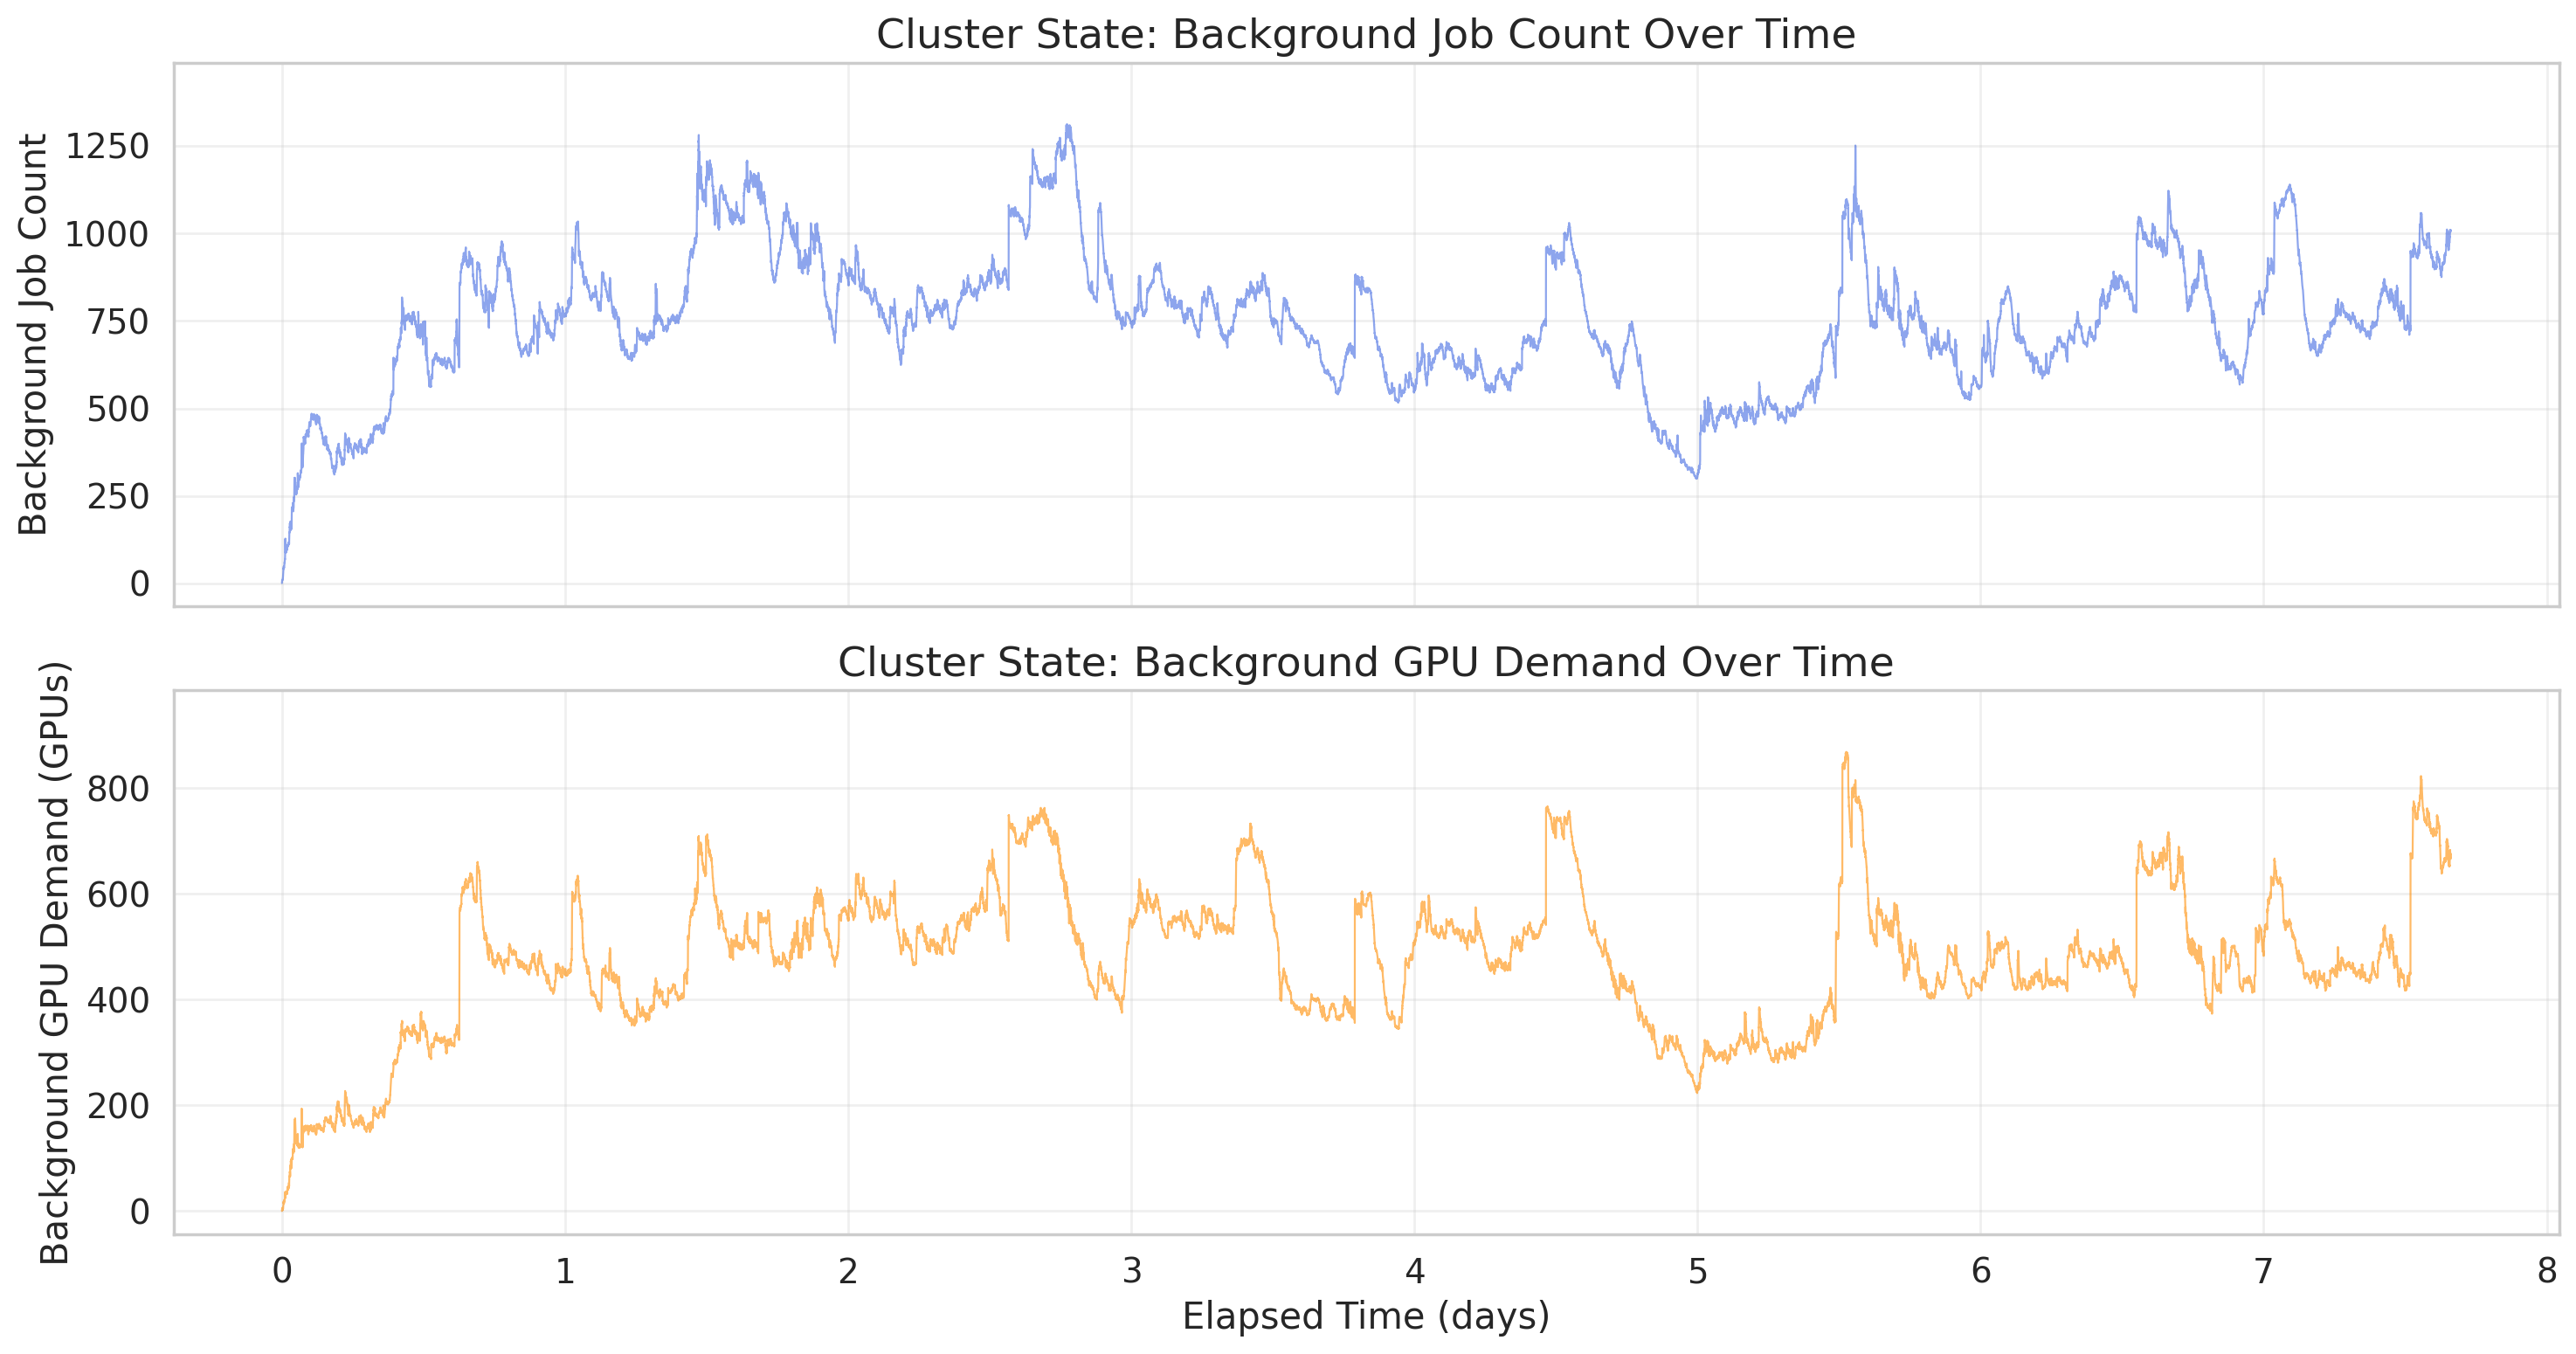
\includegraphics[width=\textwidth]{figures/nb03-fig01-cluster-load.png}
\caption[Job count and GPU demand traces]{Traces for the active job count (upper panel) and the total GPU demand (lower panel) calculated using a sweep-line algorithm from an 8-day trace. Periodic daily patterns along with variable burst sizes are observed.}
\label{fig:cluster-load}
\end{figure}


\subsection{Categorical Features}

Besides the numerical features, there were two primary categorical features that provided insight into both user behavior and the physical differences in hardware. These were defined as follows:

\begin{itemize}
    \item \texttt{user}: The user who submitted the job. Users had significantly different characteristics based on their submission history, specifically job duration and job size.
    \item \texttt{gpu\_type}: This feature described the type of GPU architecture that was assigned to the job. Each type of GPU has its own unique processing throughput that will directly affect how long it takes for an executable to run.
\end{itemize}

The use of \texttt{category} data types allows LightGBM to handle both categorical variables natively, thus eliminating the need to perform one-hot encoding and the associated memory usage. All other model types (XGBoost, Random Forest, and all DL architectures) require numerical data. Therefore, the two categorical variables must be encoded using one-hot encoding.

%% ================================================================
\needspace{5\baselineskip}
\section{Final Feature Set}

Table~\ref{tab:features} shows the full collection of numeric and categorical input variables. These variables correspond exactly to the output feature matrices produced by the pipelines outlined previously.

\begin{table}[htbp]
\centering
\caption[Feature set definition]{Feature set used for runtime prediction. All feature names correspond to the variable names used in the implementation.}
\label{tab:features}
\begin{tabular}{lll}
\hline
\textbf{Feature} & \textbf{Type} & \textbf{Description} \\ 
\hline
\texttt{gpu\_demand} & Numeric & Number of GPUs requested \\ 
\texttt{num\_cpu} & Numeric & Number of CPUs requested \\ 
\texttt{num\_inst} & Numeric & Number of instances used \\ 
\texttt{arrival\_sec} & Numeric & Relative job arrival time (seconds) \\ 
\texttt{hour\_of\_day} & Numeric (0-23) & Hour of the day \\ 
\texttt{day\_of\_week} & Numeric (0-7) & Trace-relative day index (not a calendar weekday) \\
\texttt{cluster\_load\_cpu} & Numeric & Background CPU load at job arrival \\ 
\texttt{cluster\_load\_gpu} & Numeric & Background GPU load at job arrival \\ 
\texttt{active\_job\_count} & Numeric & Number of other active jobs at arrival \\ 
\texttt{user} & Categorical & Job owner \\ 
\texttt{gpu\_type} & Categorical & GPU type used \\ 
\hline
\end{tabular}
\end{table}

Figure~\ref{fig:correlation} illustrates the Pearson correlation matrix of the numeric input features and the prediction target (\texttt{job\_runtime}). Human intuition may lead one to believe that greater CPU and GPU requests should result in longer execution durations; however, the Pearson correlation coefficient values for \texttt{num\_cpu} and \texttt{gpu\_demand} are remarkably small at 0.08 and 0.05, respectively. Strong correlations exist among the sweep-line cluster utilization features (\texttt{cluster\_load\_cpu}, \texttt{cluster\_load\_gpu}, \texttt{active\_job\_count}) up to a value of 0.89, demonstrating that these features describe the same cluster load phenomenon. Importantly, no single feature exhibits a strong linear relationship with the target variable. The lack of linear predictability provides the mathematical basis to deploy nonlinear predictors - specifically tree-based ensemble predictors (XGBoost, LightGBM, Random Forest) and deep neural networks (CNN, LSTM).

\begin{figure}[htbp]
\centering
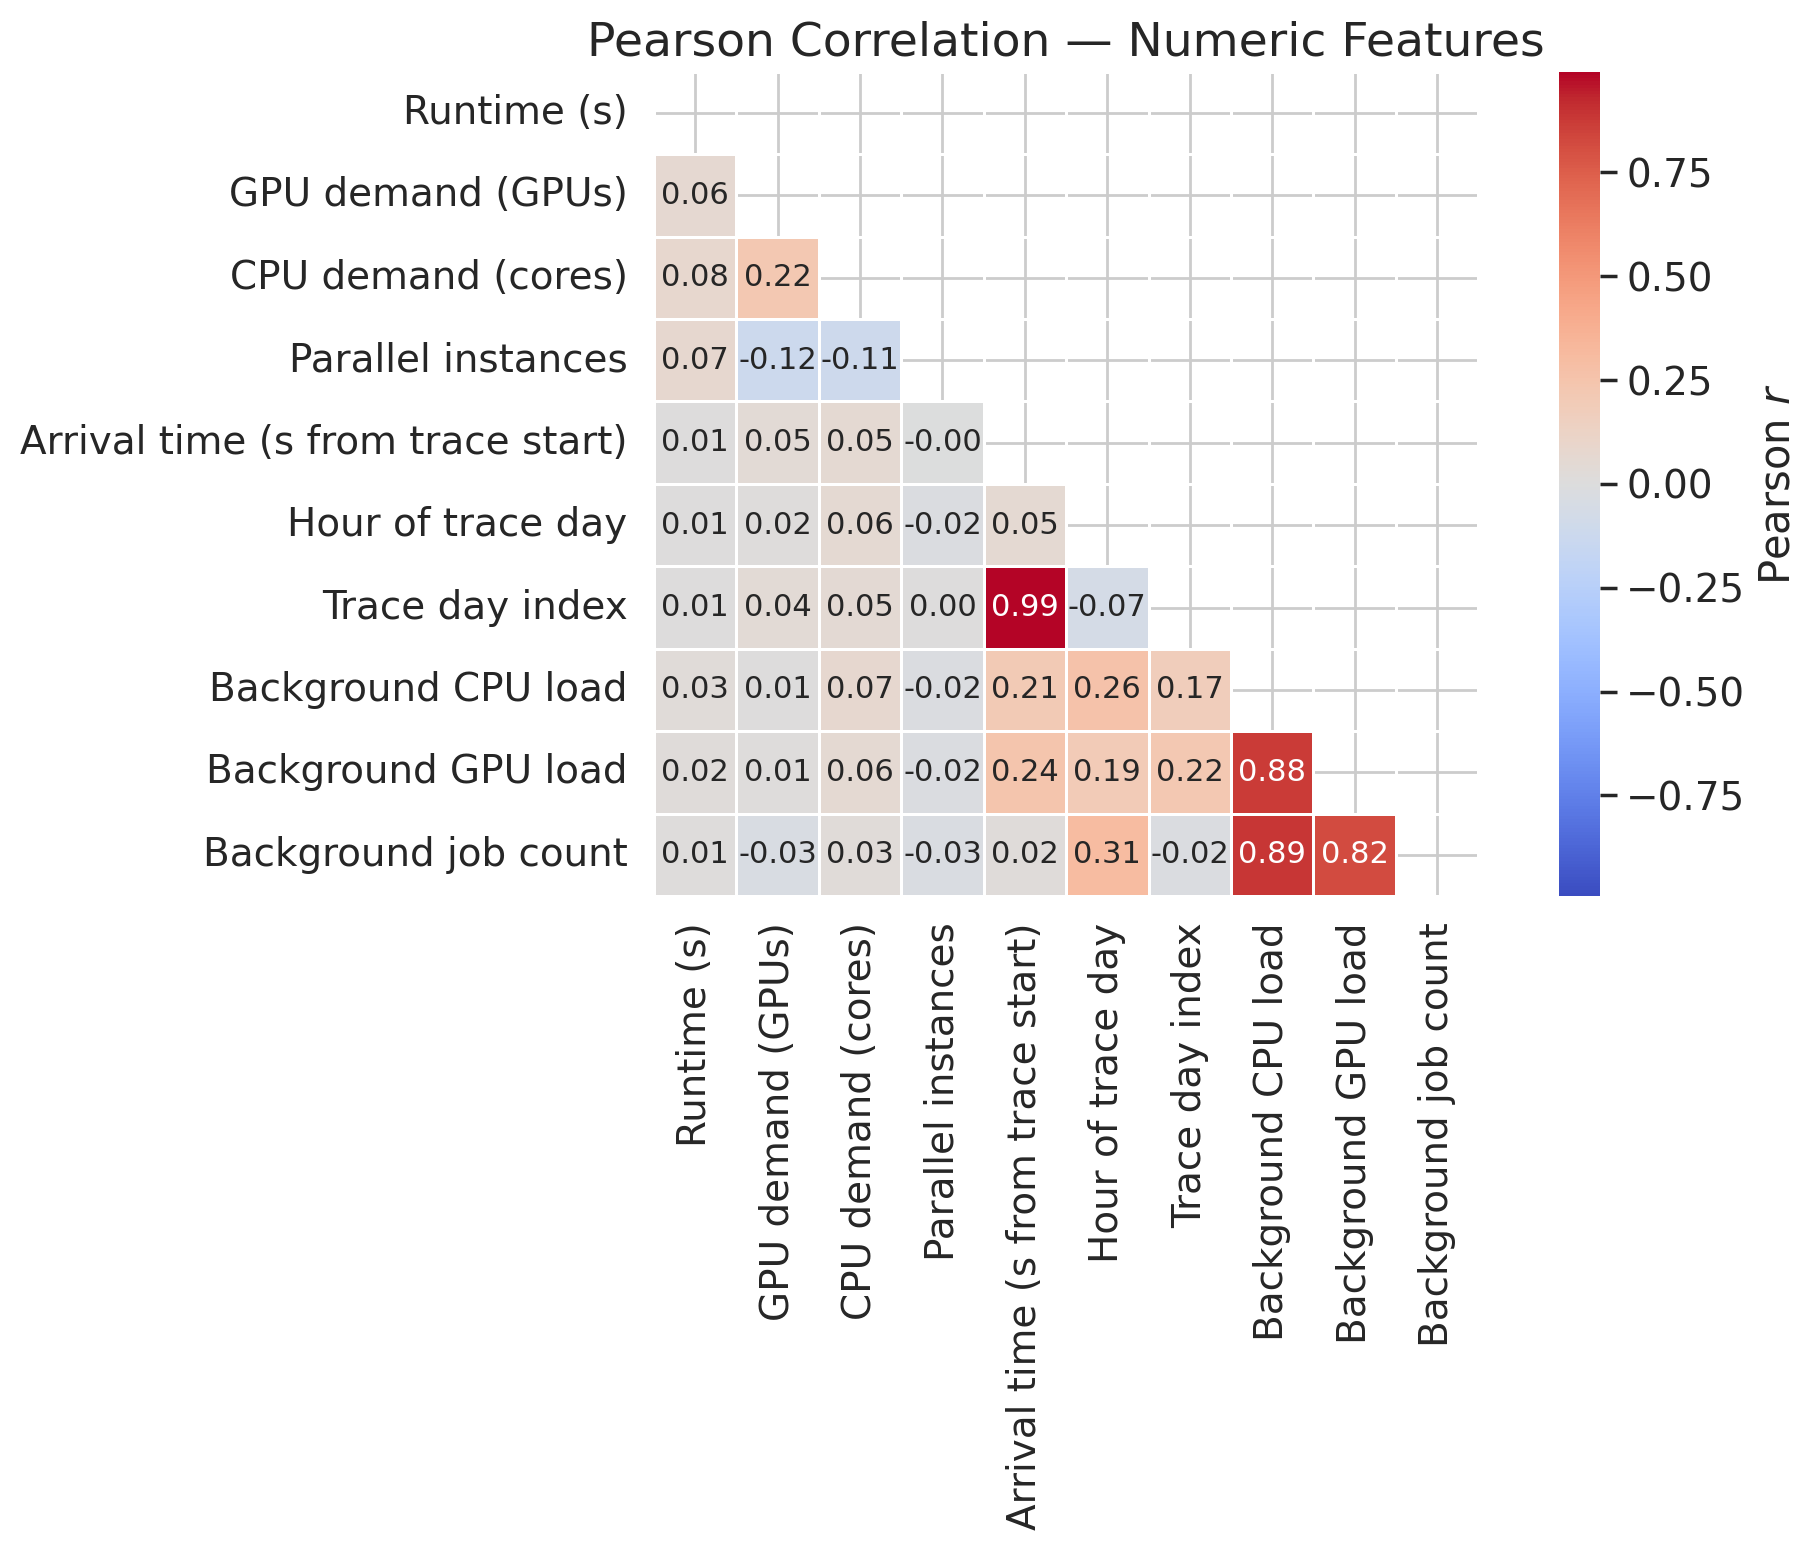
\includegraphics[width=\textwidth]{figures/nb03-fig02-correlation.png}
\caption[Pearson correlation matrix]{Pearson correlation matrix between the numeric attributes and the target variable (\texttt{job\_runtime}). None of the variables are strongly correlated to \texttt{job\_runtime}, which supports the need for non-linear regression models.}
\label{fig:correlation}
\end{figure}

\clearpage
%% ================================================================
\needspace{5\baselineskip}
\section{Data Splitting Strategy}

Temporal information leakage should be avoided when dealing with time-ordered datasets. Randomly dividing the dataset into a training and testing set will provide an artificial advantage, as a model can learn from future samples and then use those samples to predict past observations. The results will also overestimate how well the model performs compared to its ability to make predictions outside of this controlled environment.

Thus, we sort the 82,184 jobs based upon their submission times. Then we take the first 80\% (65,747 jobs) of these jobs and place them into our training set. We reserve the last 20\% (16,437 jobs) for our testing set. The fact that there exists a strictly chronological separation between the two sets provides us with the assurance that each of the jobs within our testing set was submitted \textit{after} all of the jobs within the training set. Therefore, we have established a way to simulate a real-world scenario where a scheduler uses historical data to predict the runtime of new incoming jobs.

We apply this method consistently throughout all experiments detailed in Chapter~\ref{chp:prediction}. As such, each of the models being tested is subjected to exactly the same temporal constraints. All metrics generated through evaluation against our test set are therefore unbiased measures of a model's performance once placed into production.